\chapter{Computational methods in fluid dynamics}
  In this section we shall consider an initial-boundary value problem for the system of equations in the space-time cylinder $Q_T = \Omega \times \lo 0, T \ro$, where $\Omega\in\mathbb{R}^2$.
We give here a short overview of methods for discretization in space.
	\section{Triangulation}
			  First step in the process of the discretization is to divide the computational domain $\overline{\Omega}$ into a finite number of subsets with properties described below. These subsets form the set, further denoted by $\mc{T}_h$, called the \textit{triangulation of the domain $\Omega$}. The parameter $h>0$ of the triangulation usually represents maximum of diameters of all elements $K\in\mc{T}_h$. The elements $K\in\mc{T}_h$ are in the context of the finite volume method called $finite\ volumes$.
		  \\\ \\Properties of $\mc{T}_h$:
		  \begin{enumerate}
		  \item Each $K\in\mc{T}_h$ is closed and connected with its interior $K^{\circ}\neq\emptyset$.
		  \item Each $K\in\mc{T}_h$ has a Lipschitz boundary.
		  \item$\cup_{K\in\mc{T}_h}K\,=\,\overline{\Omega}$
		  \item If $K_1,K_2\in\mc{T}_h$, $K_1\neq{K_2}$, then $K_1^{\circ}\cap{T}_2^{\circ} = \emptyset$.
		  \end{enumerate}
		  \paragraph{}
		  In our case of the two-dimensional problem, we assume that the domain $\Omega$ is obtained as an approximation of the original computational domain (also denoted by $\Omega$), and the triangulation is chosen accordingly to the following attributes:
		  \renewcommand{\labelenumi}{\Alph{enumi})}
		  \begin{enumerate}
		  \item Each $K\in\mc{T}_h$ is a closed triangle or quadrilateral, possibly with curved edges.
		  \item For $K_1,K_2\in\mc{T}_h,\,K_1\neq{K}_2$ we have either $K_1\cap{K}_2 = \emptyset$ or $K_1,K_2$ share one edge (if the shared edge is a whole common edge, we call the triangulation \emph{regular}) or $K_1,K_2$ share one vertex.
		  \item$\cup_{K\in\mc{T}_h}K\,=\,\overline{\Omega}.$
		  \end{enumerate}
		  Furthermore
		  $$
		  \mc{T}_h = \left\{K_i, i\in I\right\},
		  $$
		  where $I\subset Z^+ = \left\{0, 1, 2, ...\right\}$ is a suitable index set.\\
		  By $\Gamma_{ij}$ we denote a common edge between two
		  neighboring elements $K_i$ and $K_j$. We set 
		  $$s
		  \lo i\ro = \left\{j\in I; K_j \text{ is a neighbor of } K_i\right\}.
		  $$
		  The boundary $\partial\Omega$ is formed by a finite number of faces of elements $K_i$ adjecent to
		  $\partial\Omega$. We denote all these boundary edges by $S_j$, where $j\in I_b\subset Z^{-} = \left\{-1, -2, ...\right\}$.
		  Now we set 
		  $$
		  \gamma\lo i \ro = \left\{j\in I_b; S_j \text{ is a face of } K_i\in\mc{T}_h\right\}
		  $$ 
		  and 
		  $$
		  \Gamma_{ij} = S_j\text{ for } K_i\in \mc{T}_h\text{ such that }S_j\subset\partial K_i, j\in I_b.
		  $$
		  For $K_i$ not containing any boundary face $S_j$ we set $\gamma\lo i \ro = \emptyset$.\\
		  Obviously, $s\lo i \ro \cup\gamma\lo i\ro = \emptyset$ for all $i\in I$. If we write $S\lo i \ro = s \lo i\ro \cup \gamma\lo i \ro$, we have
		  $$
		  \partial K_i = \cup_{j\in S\lo i \ro}\Gamma_{ij},\ \ \ \partial K_i\cap\partial{\Omega} = \cup_{j\in\gamma\lo i \ro}\Gamma_{ij}.
		  $$
\ \\
\paragraph{Model example}
\label{par:model_example}
Our model example in this chapter will be the scalar \emph{linear advection-diffusion equation} with diffusion term left out:
\be
\label{ade}
\nabla \cdot \bs{f}\lo u\lo x_1, x_2\ro\ro = 0.
\ee
In particular, we will be concerned with the case 
$$\bs{f}\lo u \ro = \beta u,$$
where $\beta \lo x_1, x_2\ro = (-x_2, x_1) / \left|\bs{x}\right|$ represents a circular counterclockwise flow field and $\Omega = [0, 1] \times [0, 1]$. We prescribe the following boundary condition:
\begin{eqnarray}
u & = & g\ on\ \Gamma_-, \text{ where} \\
g & = & 1\ on\ \Gamma_-^1, \text{ and} \\
g & = & 0\ on\ \Gamma_-^2,
\end{eqnarray}
where $\Gamma_- = \left\{\bs{x} = \lo x_1, x_2\ro:\ \beta\lo x_1, x_2 \ro \cdot \bs{n}(\bs{x}) < 0\right\},\ \Gamma_1 = [0,0.5] \times {0}$, and $\Gamma_-^2 = \Gamma_-\ \backslash\ \Gamma_-^1$. We do not prescribe any boundary condition on the rest of the boundary, i.e. on $\Gamma = \partial\Omega / \Gamma_-$.
	\section{Finite Volume method}
		\subsection{Scheme derivation}
Let us assume that $u\ :\ \overline{\Omega} \rightarrow \mathbb{R}$ is a classical $\lo\mc{C}^1\ro$ solution of the equation~\eqref{ade}, $\mc{T}_h = \left\{K_i\right\}_{i\in I}$ is the finite volume mesh as an approximation of $\Omega$. Integrating the equation~\eqref{ade} over $K_i$ and using Green's theorem on $K_i$, we get the identity
\be
\int_{\partial K_i}\bs{f}\lo u\ro \cdot \bs{n} dS = 0.
\ee
Now we shall approximate the integral averages $\int_{K_i} u\lo\bs{x}\ro d\bs{x} / \left|K_i\right|$ of the quantity $u$ over the finite volume $K_i$ by $u_i$:
\be
u_i \approx \frac{1}{\left|K_i\right|}\int_{K_i}u\lo\bs{x}\ro d\bs{x},
\ee
called the value of \itshape the approximate solution \upshape on $K_i$. Futher, we approximate the flux $\bs{f}\lo u \ro \lo\bs{n}_{ij}\ro$ of the quantity $u$ through the edge $\Gamma{ij}$ in the direction $\bs{n}_{ij}$ with the aid of a \itshape numerical flux \upshape $\bs{H}\lo u_i, u_j, \bs{n}_{ij}\ro$, depending on the value of the approximate solution $u_i$ on the finite volume $K_i$, the value $u_j$ on $K_j$, and on the normal $\bs{n}_{ij}$.
If $\Gamma_{ij}\subset\partial\Omega$ (i.e. the finite volume $K_i$ is adjacent to $\partial\Omega,\ j\in\gamma\lo i \ro$), then there is no neighbor $K_j$ of $K_i$ adjacent to the face $\Gamma_{ij}$ from the exterior of $\Gamma$, and it is necessary to specify $u_j$ on the basis of boundary conditions. This will be explained further in the section about the discretization of the Euler equations.
\paragraph{}
The scheme is also equipped with $initial\ conditions\ u^0_i$, $i\in I$, defined by
\be
u_i^0 = \frac{1}{\left|K_i\right|}\int_{K_i} u^0\lo \bs{x} \ro d\bs{x},
\ee
under the assumption that the function $u^0$ from~\eqref{initial} is locally integrable, i.e. that $u^0\in L_{\text{loc}}^1\lo\Omega\ro$.
		\subsection{Properties of the numerical flux}
\label{subsec:numflux_properties}
In what follows, we shall assume that the numerical flux $\bs{H}$ has the following properties:
\begin{enumerate}
\item $\bs{H}\lo u, v, \bs{n}\ro$ is defined and continuous on $\mc{D} \times \mc{D} \times \mc{S}_1$, where $\mc{D}$ is the domain of definition of the flux $\bs{f}$ and $\mc{S}_1$ is the unit sphere in $\mathbb{R}^N$ (here $N = 2$).
\item $\bs{H}$ is $consistent$:
$$
 \bs{H}\lo u, u, \bs{n}\ro = \bs{f}\lo u\ro \bs{n},\ u\in\mc{D},\ \bs{n}\in\mc{S}_1.
$$
\item $\bs{H}$ is $conservative$:
$$
 \bs{H}\lo u, v, \bs{n}\ro = -\bs{H}\lo v, u, -\bs{n}\ro,\ u, v\in\mc{D},\ \bs{n}\in\mc{S}_1.
$$
\end{enumerate}
\ \\
\itshape We define a finite volume approximate solution of~\eqref{ade} as piecewise constant function $u_h$, defined a.e. in $\Omega$ so that $u_h|_{{K_i}^o} = u_i$ for all $i\in I$, where ${K_i}^o$ is the interior of $K_i$, i.e. ${K_i}^o = K_i \backslash \partial K_i$, and $u_i$ are obtained from the formula
\be
\label{fvm_formula}
\frac{1}{K_i}\sum_{j\in S\lo i \ro} \bs{H}\lo u_i, u_j, \bs{n}_{ij}\ro = 0,\ \ K_i\in\mc{T}_h.
\ee
The number $u_i$ is the value of the approximate solution on the finite volume $K_i$.
\upshape
		\subsection{Example}
Now we give an example of a numerical flux, which is the $upwinding$ numerical flux defined by
\be
\label{upwinding_flux}
H\lo u_i, u_j, n_{ij}\ro = \begin{cases} u_i, & \mbox{if } \beta\cdot\bs{n}_{ij} > 0 \\ u_j, & \mbox{if } \beta\cdot\bs{n}_{ij} \leq 0 \end{cases}.
\ee
Solutions of the model example using the finite volume method with the numerical flux~\eqref{upwinding_flux} are presented below. The computation was obtained on three different meshes.

\begin{figure}[H]
\begin{center}
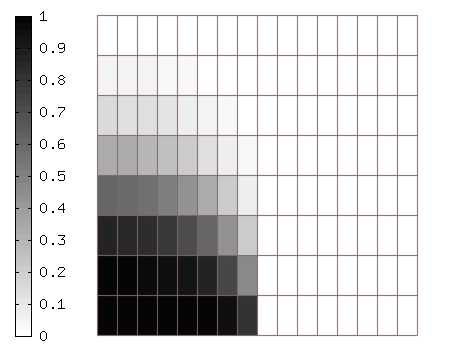
\includegraphics[width=0.48\textwidth]{minor_examples/FVM00.png}\ \ \ 
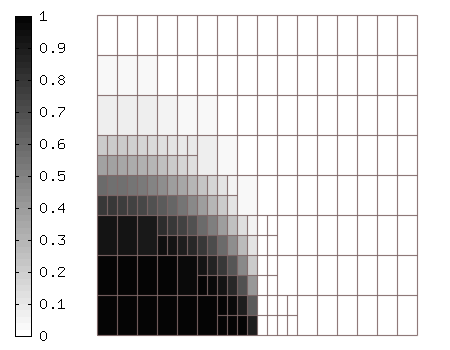
\includegraphics[width=0.48\textwidth]{minor_examples/FVM01.png}
\end{center}
\vspace{-4mm}
\caption{Solution $u$ on a mesh with 128 (left), and 206(right) elements.}
\end{figure}

\begin{figure}[H]
\begin{center}
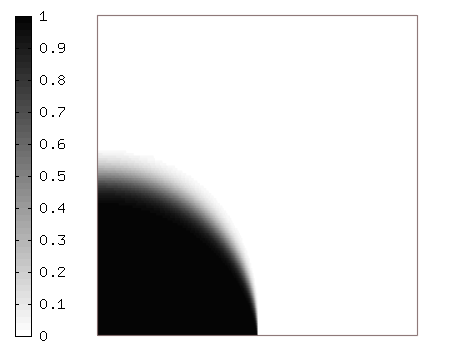
\includegraphics[width=0.48\textwidth]{minor_examples/FVM02.png}\ \ \ 
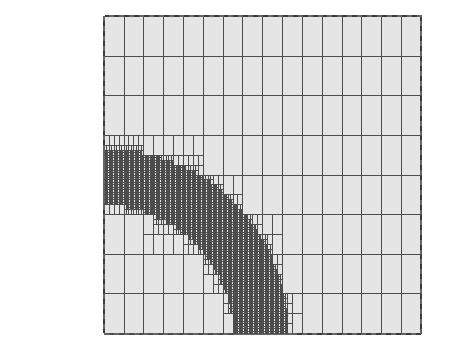
\includegraphics[width=0.48\textwidth]{minor_examples/FVM02Mesh.png}
\end{center}
\vspace{-4mm}
\caption{Solution $u$ (left) and the corresponding mesh (right) with 4751 elements.}
\end{figure}
We can see that the solution is smeared near the steep gradient. We would like to avoid this.
	\section{Finite Element Method}
Application of the standard FEM to the problem~\eqref{ade} is very straightforward. We multiply the equation~\eqref{ade} with a test function $v$ from a suitable finite-dimensional approximation of the $H^1\lo\Omega\ro$ space. We then integrate over $\Omega$ and use the Green's theorem. We get the following identity:
\be
\int_{\Omega}\bs{f}\lo u\ro \cdot \nabla v d\bs{x} = \int_{\Gamma_-}g v\ dS,
\ee
which must hold for all $v$ from the finite-dimensional approximation of the $H^1\lo\Omega\ro$ space. 
As this finite-dimensional sub-space of the $H^1\lo\Omega\ro$ space, we usually take the space of continuous functions, which are polynomials up to order $p$ on each element of the triangulation.
\paragraph{}
For singularly perturbed equations, or strictly first order equaions, such as our model equation, the standard Galerkin FEM exhibits $Gibbs$ $phenomenon$, manifested by $spurious$ $oscillations$ in the numerical solution. This behavior is well noticeable in the following figures.
		\subsection{Example}
\begin{figure}[H]
\begin{center}
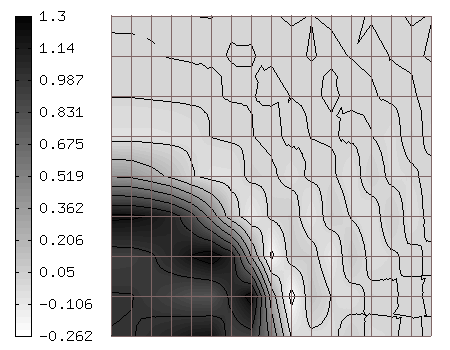
\includegraphics[width=0.48\textwidth]{minor_examples/FEM00.png}\ \ \ 
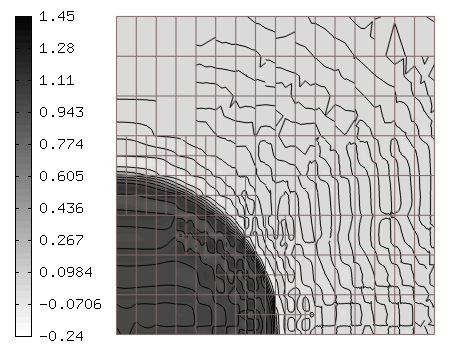
\includegraphics[width=0.48\textwidth]{minor_examples/FEM01.png}
\end{center}
\vspace{-4mm}
\caption{Solution $u$ on a mesh with 128 elements and p = 1 (left), and 206 elements and p = 2 (right).}
\end{figure}

\begin{figure}[H]
\begin{center}
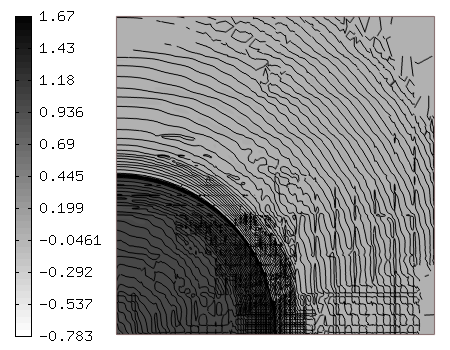
\includegraphics[width=0.48\textwidth]{minor_examples/FEM02.png}\ \ \ 
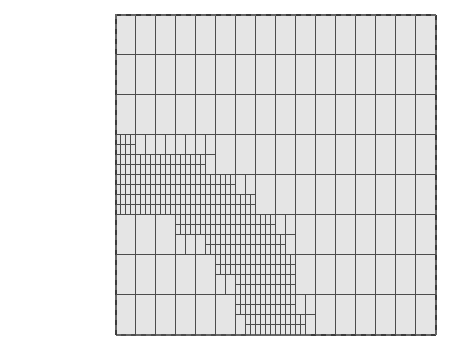
\includegraphics[width=0.48\textwidth]{minor_examples/FEM02Mesh.png}
\end{center}
\vspace{-4mm}
\caption{Solution $u$ (left) and the corresponding mesh (right) with 449 elements, p = 5, and 11206 degrees of freedom.}
\end{figure}
	The oscillations can be diminished using stabilization technique, e.g. streamwind-upwind petrov-galerking stabilization. Their disadvantage is the necessity to fine tune various parameters for them to function properly. For a reference, see e.g.~\cite{Knobloch_1},~\cite{Knobloch_2},~\cite{SUPG}.

	\section{Discontinuous Galerkin method}
\label{sec:DG}
For complex problems of compressible flow, the choice of optimal stabilization parameters becomes quite sophisticated and difficult. Due to this reason, there  was an effort to develop methods which would not need such stabilization techniques, and would still offer reasonable resolution of shockwaves, boundary and interior layers, and steep gradients without exhibiting spurious oscillations in an approximate solution. It is based on the idea to combine finite volume and finite element methods leading to the so-called \emph{discontinuous Galerkin finite element method (DGFEM)}. Here we shall derive and analyze DGFEM for our model example. Let $\mc{T}_h$ be a triangulation of $\Omega$. For each $K\in\mc{T}_h$ we introduce the notation
\begin{eqnarray}
\partial K^- & = & \left\{x\in\partial K;\beta\lo\bs{x}\ro\cdot\bs{n}\lo\bs{x}\ro <0\right\},\\
\partial K^+ & = & \left\{x\in\partial K;\beta\lo\bs{x}\ro\cdot\bs{n}\lo\bs{x}\ro \geq 0\right\}.
\end{eqnarray}
By $H^k\lo\Omega, \mc{T}_h\ro$ we denote the so-called \itshape broken Sobolev space\upshape:
\be
H^k\lo\Omega,\mc{T}_h\ro = \left\{v\in L^2\lo\Omega\ro;\ v|_K\in H^k\lo K\ro \forall K\in \mc{T}_h\right\}.
\ee
For $u\in H^1\lo\Omega,\mc{T}_h\ro$ we set
\be
u_K^+ = \text{trace of } u|_K \text{ on }\partial K
\ee
(i.e. the interior trace of $u$ on $\partial K$). For each edge $E\subset\partial K\backslash\Gamma$ of $K$, there exists $K'\neq K,\ K'\in\mc{T}_h$, adjacent to $E$ from the opposite side than $K$. Then we put
\be
u_K^- = \text{trace of } u|_{K'} \text{ on } E.
\ee
In this way we obtain the exterior trace $u_K^-$ of $u$ on $\partial K\backslash\Gamma$ and define the jump of $u$ on $\partial K\backslash\Gamma$:
\be
[u]_K = u_K^+ - u_K^-.
\ee
\subsection{Derivation of the DGFEM}
		Let $u\in H^1\lo\Omega\ro$ be a solution of the problem~\eqref{ade}. Then $u$ satisfies the identity
\be
\int_K \nabla\cdot\lo\beta u\ro\varphi d\bs{x} = 0,\ \ \varphi\in H^1\lo\Omega,\mc{T}_h\ro,\ K\in\mc{T}_h.
\ee
The application of Green's theorem gives
\begin{eqnarray}
\label{upwinding_derivation_ade}
\int_K \nabla\cdot\lo\beta u\ro\varphi d\bs{x} 
& = & \int_{\partial K}\lo\beta u_K^+\ro\cdot\bs{n}\varphi_K^+ dS - \int_K \lo\beta u\ro\cdot\nabla \varphi d\bs{x}\\\nonumber
& = & \int_{\partial K^-}\lo\beta u_K^+\ro\cdot\bs{n}\varphi_K^+ dS + \int_{\partial K^+}\lo\beta u_K^+\ro\cdot\bs{n}\varphi_K^+ dS\\\nonumber
& - & \int_K \lo\beta u\ro\cdot\nabla \varphi d\bs{x},
\end{eqnarray}
where $\bs{n}$ is the unit outer normal to the element boundary $\partial K$. As $u\in H^1\lo\Omega\ro$, we have $u_K^- = u_K^+$. Moreover, $u_K^-|_{\partial K^-\cap\Gamma}:=u|_{\partial K^-\cap\Gamma} = g$. 
Then we can write
\begin{eqnarray}
\int_K \nabla\cdot\lo\beta u\ro\varphi d\bs{x} & = & \int_{\partial K^-}\lo\beta u_K^-\ro\cdot\bs{n}\varphi_K^+ dS + \int_{\partial K^+}\lo\beta u_K^+\ro\cdot\bs{n}\varphi_K^+ dS\\\nonumber & - & \int_K \lo\beta u\ro\cdot\nabla \varphi d\bs{x}.
\end{eqnarray}
Applying Green's theorem again, we get the identity
\be
\label{DG_identity_ade}
\int_K \nabla\cdot\lo\beta u\ro\varphi d\bs{x} = \int_{\partial K^-}\lo\beta \lo u_K^+ - u_K^-\ro\ro\cdot\bs{n}\varphi_K^+ dS.
\ee
Setting
\begin{eqnarray}
a_K\lo u, \varphi\ro & = & \int_K \nabla\cdot\lo\beta u\ro\varphi d\bs{x} - \int_{\partial K^-\backslash\Gamma}\lo\beta [u]_K\ro\cdot\bs{n}\varphi_K^+ dS\\\nonumber & - & \int_{\partial K^-\cap\Gamma_-}\lo\beta u_K^+\ro\cdot\bs{n}\varphi_K^+ dS,
\end{eqnarray}
\be
L_K\lo\varphi\ro = \int_{\partial K^-\cap\Gamma_-}\lo\beta g\ro\cdot\bs{n}\varphi_K^+ dS,
\ee
we can rewrite the equation~\eqref{DG_identity_ade} as
\be
\label{final_DG_ade}
a_K\lo u, \varphi\ro = L_K\lo\varphi\ro,\ \ \varphi\in H^1\lo K\ro,\ \ K\in\mc{T}_h.
\ee
This identity makes sense also for $u\in H^1\lo\Omega, \mc{T}_h\ro$. In this case, we can note that in~\eqref{upwinding_derivation_ade}, on $\partial K^-$ (= the inlet of $K$ with respect to the velocity $\beta$) we replace the value $u_K^+$ (the interior trace of u) by $u_K^-$. This means that $upwinding$ is used here, because the value of the trace of $u$ on $\partial K^-$ is taken from the side of $\partial K^-$ against the velocity direction.
\paragraph{}
Now, on the basis of~\eqref{final_DG_ade} we come to the definition of the $discrete\ problem$. The $approximate\ solution$ is a function $u_h$ satisfying the conditions
\begin{enumerate}
\item $u_h\in S_h = S^{p, -1}\lo\Omega,\mc{T}_h\ro:=\left\{\varphi\in L^2\lo\Omega\ro;\varphi|_K\in P^p\lo K\ro\forall K \in \mc{T}_h\right\}$
\item $a_K\lo u_h, \varphi_h\ro = L_K\lo\varphi_h\ro,\ \forall\varphi_h\in S_h,\ \forall K\in\mc{T}_h$.
\end{enumerate}
Here, $p$ is an integer. In general on each element a different polynomial degree can be used for the approximation. The approximate solution and test functions are piecewise polynomial functions without any continuity requirement on interfaces between neighboring elements. The continuity requirement is replaced here by the jump term $\int_{\partial K^-\backslash\Gamma}\lo\beta [u]_K\ro\cdot\bs{n}\varphi_K^+ dS$.

We can see that we successfully avoided the smeared layer close to the steep gradient, and also the Gibbs phenomenon in the whole domain. What we have to deal here with on the other hand are overshoots and undershoots close to the step gradient. There is several approaches, some of which are described in the last chapter with numerical experiments, for the case of the Euler equations.
\subsection{Example}
\begin{figure}[H]
\begin{center}
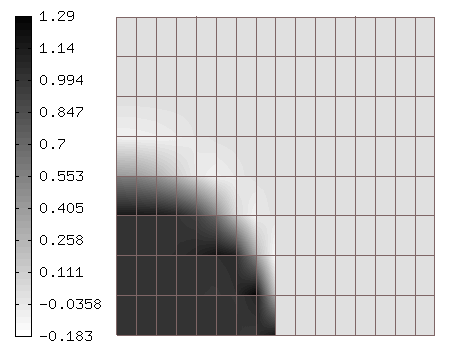
\includegraphics[width=0.48\textwidth]{minor_examples/DG00.png}\ \ \ 
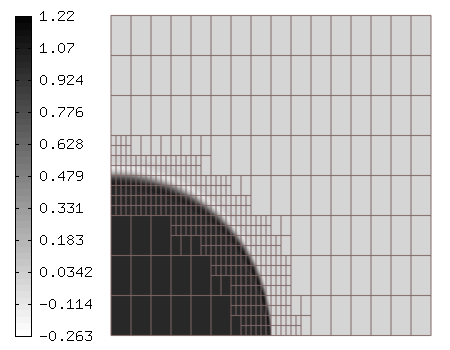
\includegraphics[width=0.48\textwidth]{minor_examples/DG01.png}
\end{center}
\vspace{-4mm}
\caption{Solution $u$ on a mesh with 128 elements and p = 1 (left), and 206 elements and p = 2 (right).}
\end{figure}

\begin{figure}[H]
\begin{center}
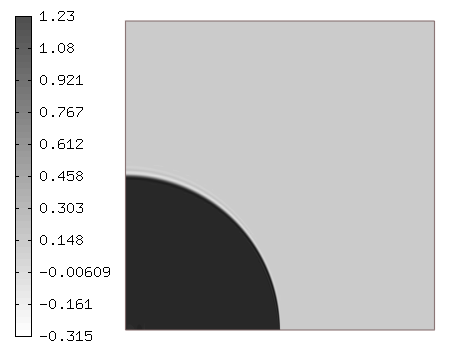
\includegraphics[width=0.48\textwidth]{minor_examples/DG02.png}\ \ \ 
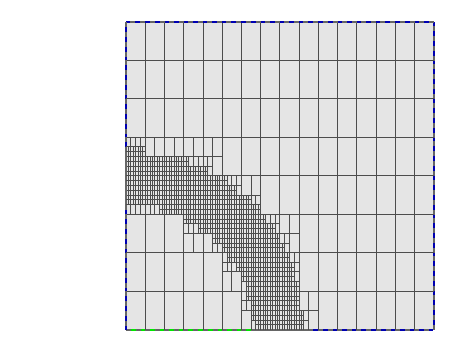
\includegraphics[width=0.48\textwidth]{minor_examples/DG02Mesh.png}
\end{center}
\vspace{-4mm}
\caption{Solution $u$ (left) and the corresponding mesh (right) with 1271 elements, p = 3, and 20336 degrees of freedom.}
\end{figure}
